\section*{Motivation}
Efficient team schedule planning is a complex challenge, particularly in organizations that require real-time coordination and resource management.
Existing scheduling services often have significant limitations, such as proprietary nature, lack of customization, and dependence on third-party infrastructure.
This highlights the need for tailored solutions that can address specific organizational requirements more effectively.
This project aims to develop a self-hosted open-source booking system designed for organizations that need a private, adaptable scheduling solution.
The system will provide a web-based interface where users can:
\begin{itemize}
    \item Make and manage reservations
    \item Check real-time room availability
    \item  Filter bookings by person or room
    \item View all reservations on a centralized calendar
\end{itemize}

The backend will be built using the Spring Framework, ensuring scalability, security, and ease of integration with existing infrastructure.
Unlike cloud-based alternatives, this system will store all data locally, giving organizations complete privacy and control over scheduling information.
By combining flexibility, transparency, and data privacy, this project can provide a practical alternative to commercial scheduling tools, empowering organizations with greater autonomy and customization options.
\addcontentsline{toc}{section}{Motivation}


\pagestyle{headings}
Here we will talk about why the calendar is needed

Firstly, lets take a look at the current solution used by my university,CTU. Rozvrh.fjfi.cvut.cz is a website where students can see their schedule.
\section{The current solution}\label{sec:the-current-solution}
\begin{figure}[h]
  \centering
  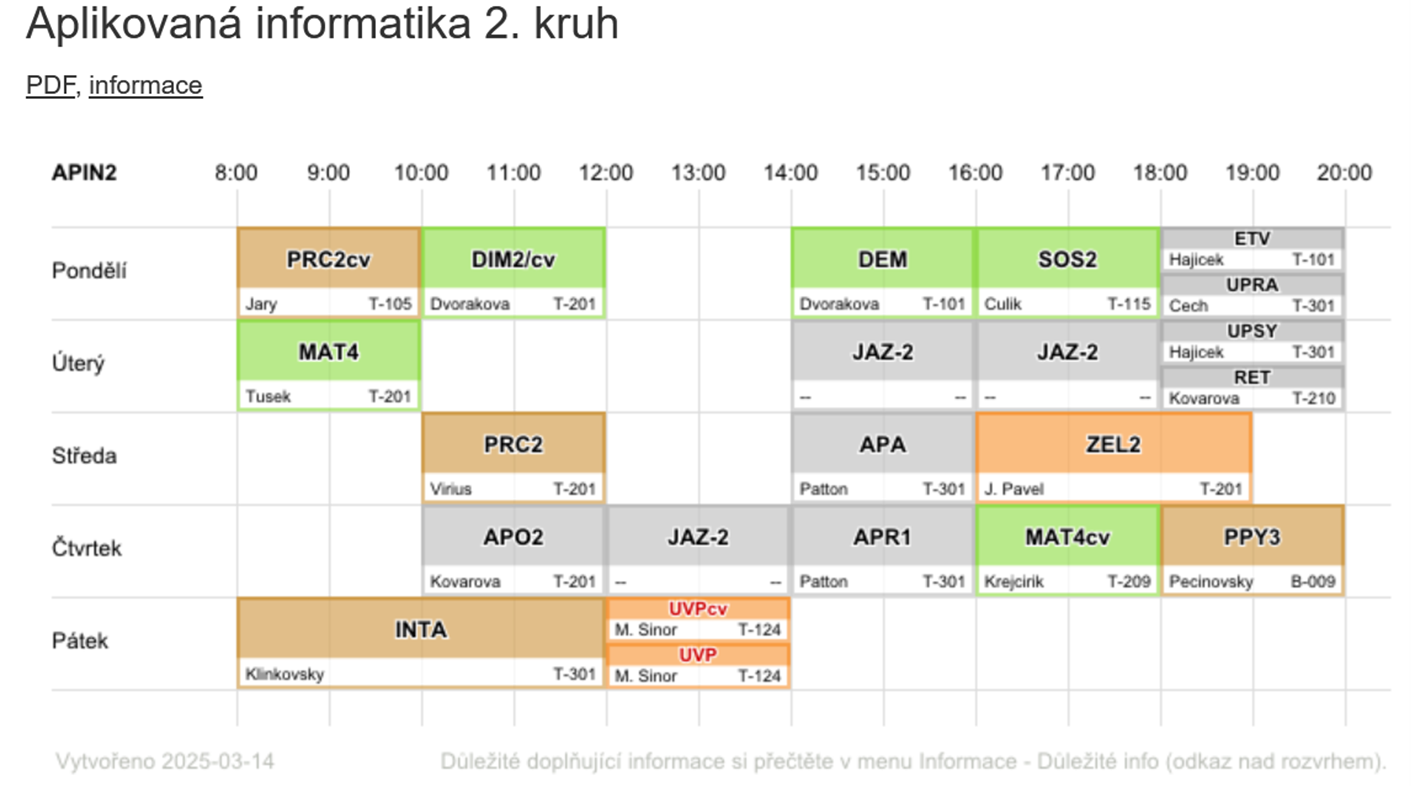
\includegraphics[width=0.6\textwidth]{img}
  \caption{Screenshot of the current solution}
  \label{fig:rozvrh}
\end{figure}

It can be seen on~\ref{fig:rozvrh} that while the website completes its main purpose, it is not customizable, which makes it hard to use.
For example, if a student has a class that is from another year or/and program, they have to look at another picture and manually compare them.
From my experience, many students have screenshots on their phones and they cross-out the classes that they are not registered to.
They may have a few screenshots, for different programs or years.
It is not a good solution, as it allows for misunderstandings and mistakes.

This is why a project focused on creating a calendar that is easy to use and customizable is needed.
\section{The solution}\label{sec:the-solution}
\begin{figure}[h]
  \centering
  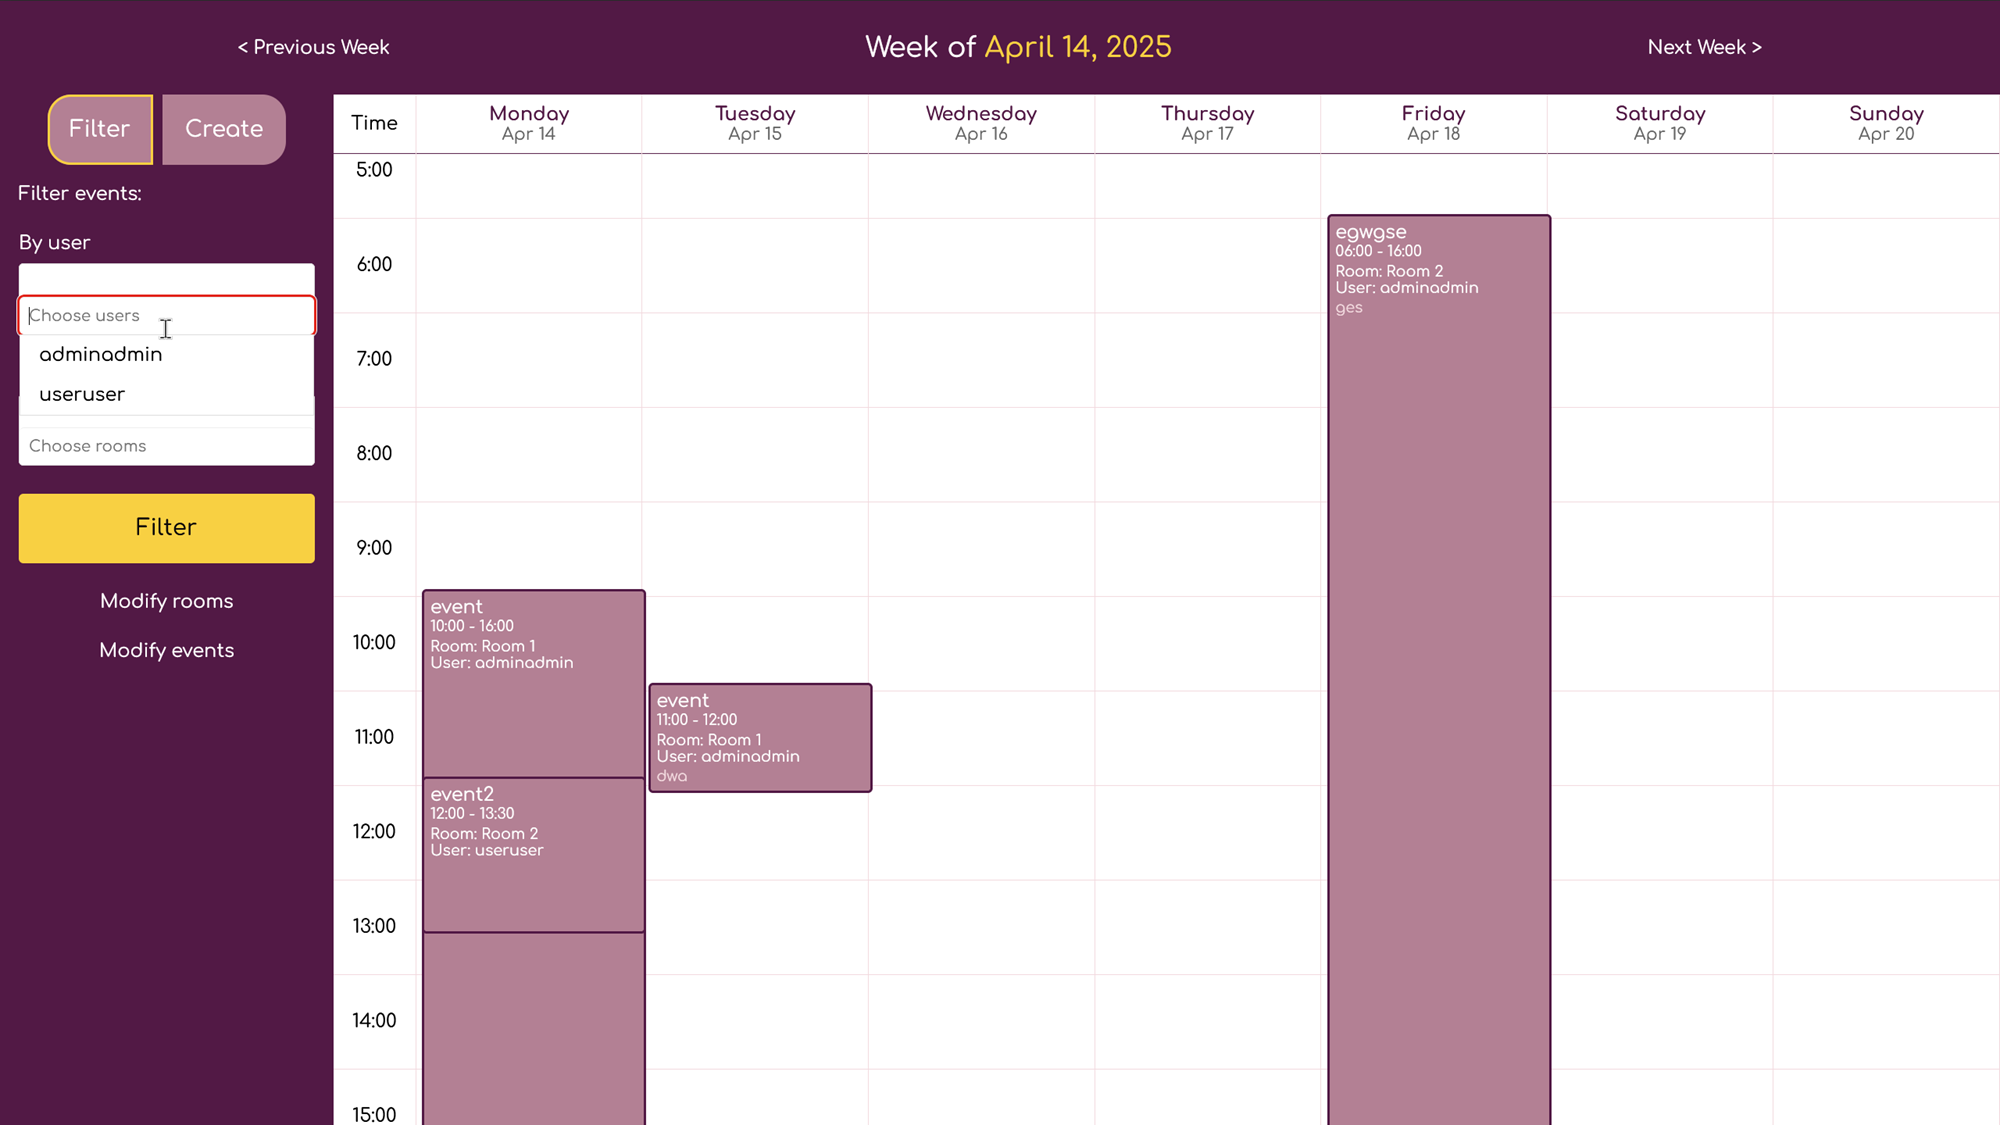
\includegraphics[width=0.6\textwidth]{TeamJob}
  \caption{Screenshot of the new solution}
  \label{fig:TeamJob}
\end{figure}
TeamJob is a web application that allows users to filter exactly what they want to see.
By default, all the events that are happening this week are shown.
The user can filter the events by the room and the person that is assigned to this event.
This allows for a more precise view of the calendar, where the user can see only the events that are important to them.
The user can also move between weeks.
A specific day-view allows the user to see the events that are happening on a specific day, if there are too many events to show them all at once.

